\section{缀加平面波(Augmented Plane Wave, APW)方法}
APW是Slater提出MT球近似时设计的周期体系的波函数展开方法\cite{PR51-846_1937,PR91-528_1953},如图\ref{Muffin_tin_0}所示。%后来Slater又对APW方法进行“简化”\cite{}%,但实际上原始的APW思想更直接。
\begin{figure}[h!]
\centering
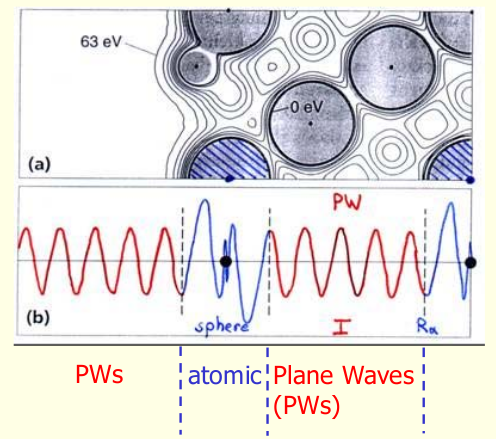
\includegraphics[height=1.10in,width=1.45in,viewport=1 20 485 435,clip]{APW.png}
\caption{\small \textrm{Partitioning of the unit cell into atomic spheres and an interstitial region.}}%(与文献\cite{EPJB33-47_2003}图1对比)
\label{Muffin_tin_0}
\end{figure}
根据MT近似,在WS原胞的每个MT球内,势能具有球对称性$V(r)$,MT球内的基函数表示为:
\begin{equation}
  \varphi(\vec k_i,\vec r)=\sum_{l=0}^{\infty}\sum_{m=-l}^lA_{lm}(\vec k_i)u_l(|\vec r-\vec r_s|)Y_{lm}(\widehat{\vec r-\vec r_s})
  \label{eq:solid-109}
\end{equation}
这里$Y_{lm}$是球谐函数;$\vec k_i=\vec k+\vec G_i$;$\vec G_i$是倒格矢;$\vec r_s$是第$s$个MT球心位置,$A_{lm}$是待定系数;$u_l(\vec r)$是径向Schr\"odinger方程
\begin{equation}
  -\frac1{r^2}\frac d{dr}\left(r^2\frac{du_l}{dr}\right)+\left[\frac{l(l+1)}{r^2}+V(r)\right]u_l=E_l'u_l
  \label{eq:solid-110}
\end{equation}
为确定$u_l(r)$,要求$u_l(r)$的边条件$r$=0是非奇异的,但在MT球面$r$=$R_{MT}^s$上,没有对$u_l(r)$加任何限制条件,因此能量式\eqref{eq:solid-110}中的$E_l'$可以取任意值。

在MT球外的间隙区,MT势能取为0,间隙区的基函数为:
\begin{equation}
	\varphi(\vec k_i,\vec r)=\exp\mathrm{i}\vec k_i\vec r=\exp\mathrm{i}\vec k_i\cdot(\vec r_s+\vec r)
  \label{eq:solid-111}
\end{equation}
将平面波用球谐函数展开,
\begin{equation}
	\exp\mathrm{i}\vec k_i\cdot\vec r=4\pi\sum_{l=0}^{\infty}\sum_{m=-l}^l\mathrm{i}^lj_l(|\vec k_i|r)Y_{lm}^{\ast}(\hat{\vec k}_i)Y_{lm}(\hat{\vec r})
  \label{eq:solid-112}
\end{equation}
这里$j_l(|\vec k_i|r)$是第$l$阶球Bessel函数;$\hat{\vec k}_i$和$\hat{\vec r}$是矢量$\vec k$和$\vec r$与$z$轴的夹角对应球坐标角度部分$\theta$和$\phi$。

为了使得基函数在球面上连续条件,要求式\eqref{eq:solid-109}和\eqref{eq:solid-111}在球面上数值相等,由此可确定系数$A_{lm}(\vec k_i)$:
$$A_{lm}(\vec k_i)=4\pi e^{\mathrm{i}\vec k_i\cdot\vec r_s}\mathrm{i}^lY_{lm}(\hat{\vec k}_i)j_l(|\vec k_i|R_{MS}^s)/u_l(E,R_{MT}^s)$$
所以APW的基组可以表示为:
\begin{equation}
  \begin{split}
    \varphi&(\vec k_i,\vec r)\\
    &=\left\{\begin{aligned}
	    &e^{\mathrm{i}\vec k_i\cdot\vec r_s}e^{\mathrm{i}\vec k_i\cdot\vec r},&|\vec r|>R_{MT}^s\\
    &4\pi e^{\mathrm{i}\vec k_i\cdot\vec r_s}\sum_{lm}\mathrm{i}^lj_l(|\vec k_i|R_{MS}^s)Y_{lm}^{\ast}(\hat{\vec k}_i)Y_{lm}(\hat{\vec r})u_l(r,E')/u_l(R_{MT}^s,E'),\quad&|\vec r|\leqslant R_{MT}^s
    \end{aligned} \right.
  \end{split}
  \label{eq:solid-113}
\end{equation}

对于基函数在MT球面不连续的情形,用Schlosser和Marcus的能量变分表达式\cite{PR131-2529_1963},
\begin{equation}
  \begin{split}
    E\int_{\mathrm{I+II}}\Psi^{\ast}\Psi dV=&\int_{\mathrm{I+II}}\Psi^{\ast}\mathbf H\Psi dV+\frac12\int_S\left[(\Psi_{\mathrm{II}}-\Psi_{\mathrm I})\frac{\partial}{\partial\rho}\Psi_{\mathrm {II}}^{\ast}+\frac{\partial}{\partial\rho}\Psi_{\mathrm I}^{\ast}\right.\\
    &-(\Psi_{\mathrm {II}}^{\ast}+\Psi_{\mathrm I}^{\ast})\left.\left(\frac{\partial}{\partial\rho}\Psi_{\mathrm{II}}-\frac{\partial}{\partial\rho}\Psi_{\mathrm I}\right)\right]dS
  \end{split}
  \label{eq:solid-114}
\end{equation}
这里I和II分别表示MT球的内(I)外(II)两部分。上式中的前两个积分项表示对整个WS原胞的积分,第三个积分项是对MT球的球面S的积分。$\partial/\partial\rho$沿球面正方向对区域I的偏导。采用连续基函数,则\eqref{eq:solid-114}可以简化为:
\begin{equation}
  \begin{split}
    E\int_{\mathrm{I+II}}\Psi^{\ast}\Psi dV=&\int_{\mathrm{I+II}}\Psi^{\ast}\mathbf H\Psi dV\\
    &-\frac12\int_S(\Psi_{\mathrm {II}}^{\ast}+\Psi_{\mathrm I}^{\ast})\left(\frac{\partial}{\partial\rho}\Psi_{\mathrm{II}}-\frac{\partial}{\partial\rho}\Psi_{\mathrm I}\right)dS
  \end{split}
  \label{eq:solid-115}
\end{equation}
这里的球面积分是考虑波函数$\Psi$在MT球面上导数不连续。

因为APW基函数径向部分与能量参数$E_l$有关,因此矩阵元与$E_l$有关。为了获得能量本征值$E_l$,必须求解$\vec k$-空间中每个点的能量$E_l$高阶行列式,该过程非常麻烦。为了克服基函数对能量$E_l$的相关,人们提出了多种线性化思想\cite{PRB2-3098_1970,PRB2-290_1970,JPF9-661_1979,PRB19-6094_1979}。线性化缀加平面波(linearized augmented plane-wave, LAPW)方法的思想是在某个给定值$E_{l0}$附近对能量作Taylor展开到一阶\cite{PRB12-3060_1975}。由于波函数的线性化引入的误差,比因为对势能近似引入的误差小得多。换句话说,通过引入线性化,可使得固体中价电子径向波函数与能量参数无关。由此得到Hamiltonian和重叠矩阵与能量参数无关。Koelling和Arbman将LAPW方法应用于Cu的计算\cite{JPF5-2041_1975}。Smr\v cka提出了二次APW方法\cite{Smrcka}。
与APW方法相似,LAPW方法的基函数取为:
\begin{equation}
  \varphi(\vec k_j,\vec r)=\left\{
  \begin{aligned}
	  &\Omega_0^{-1/2}\exp{\mathrm{i}\vec k_j\cdot\vec r},&r>R_{MT}^s\\
    &\sum_{lm}[A_{lm}u_l(E_l,r)+B_{lm}\dot u_l(E_l,r)]Y_{lm}(\hat{\vec r}),\quad&r\leqslant R_{MT}^s
  \end{aligned}\right.
  \label{eq:LAPW-basis}
\end{equation}
这里$R_{MT}^s$是MT球半径;$\vec k_j=\vec k+\vec G_j$,$\vec k$是不可约Brillouin区中的波矢;$\vec G_j$是倒空间格矢;$u_l(E_l,r)$是满足能量为$E_l$的径向Schr\"odinger方程的解波函数;$\dot u_l(E_l,r)$是解波函数对能量$E_l$的一阶导数;$Y_{lm}$是球谐函数;$\Omega_0$是WS原胞体积。与APW不同,这里$E_l$是指定范围内的能量参数,而非变量。不同的角动量$l$可指定不同的能量。关于APW/LAPW方法基函数(径向部分)在球面上的衔接如图\ref{Muffin_tin}所示。
\begin{figure}[h!]
\centering
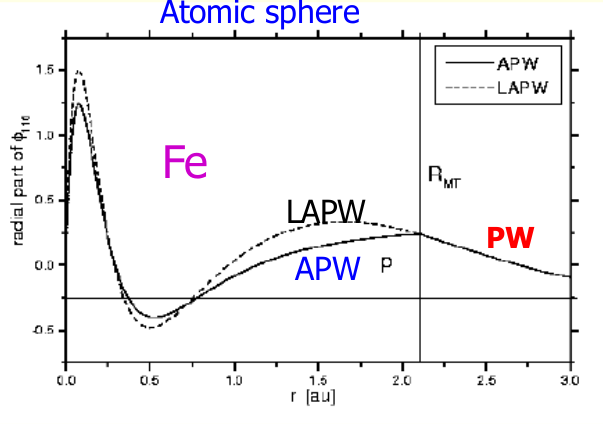
\includegraphics[height=1.30in,width=1.98in,viewport=1 20 585 435,clip]{WIEN2k-LAPW.png}
\caption{\small \textrm{Partitioning of the unit cell into atomic spheres(I) and an interstitial region(II)}}%(与文献\cite{EPJB33-47_2003}图1对比)
\label{Muffin_tin}
\end{figure}

为了提高LAPW方法的线性化程度(即提高基组的变分自由度),在同一能量范围处理半芯态(接近价态的能量较高的芯态)和价态,可采用外加基函数(与$\vec k$无关)方案,这部分外加基函数称为局域轨道(local orbitals, LO)\cite{PRB43-6388_1991,Singh}。由此构造的基函数包含两个指定能量的径向波函数和其中一个能量导数,这样的基函数即LAPW-LO:
\begin{equation}
  \phi_{lm}^{LO}(\vec r)=[A_{lm}u_l(E_{1,l},r)+B_{lm}\dot u_l(E_{1,l},r)+C_{lm}u_l(E_{2,l},r)]Y_{lm}(\hat{\vec r})
  \label{eq:LAPW-LO}
\end{equation}
根据条件$\phi_{lm}^{LO}$在MT球面上数值为零且保持一阶导数连续,并要求$\phi_{lm}^{LO}$在MT球内归一化,可以确定系数$A_{lm}$,$B_{lm}$,$C_{lm}$。

Sj\"ostedt等\cite{SSC114-15_2000}的计算表明,在标准LAPW方法中,将平面波展开使之在MT球面上与球内函数数值和一阶导数连续,这并非是实现Slater型APW方法最有效的线性化方法。采用指定能量参数$E_l$的APW形式的径向波函数[式\eqref{eq:APW-basis}],外加APW型局域轨道(local orbit, lo)扩展基函数,是更有效的方案,称为APW+lo。
\begin{equation}
  \varphi_{\vec k_i,\vec r}=\sum_{lm}[A_{lm}(\vec k_i)u_l(E_l,r)]Y_{lm}(\hat{\vec r})
  \label{eq:APW-basis}
\end{equation}
\begin{equation}
  \phi_{lm}^{lo}=[A_{lm}u_l(E_{1,l})+B_{lm}\dot u_l(E_{1,l})]Y_{lm}(\hat{\vec r})
  \label{eq:APW-lo}
\end{equation}
APW+lo基函数式\eqref{eq:APW-lo}形式上与标准LAPW式\eqref{eq:LAPW-basis}形式非常相似,但这里系数$A_{lm}$和$B_{lm}$与$\vec k$无关,是根据式\eqref{eq:APW-lo}在MT球边界上数值为零并且在MT球内归一化确定。这样构造的APW+lo基函数,总的波函数在MT球面上平滑且一阶可导的,但是根据式\eqref{eq:solid-115},在MT球面上有动能部分对Hamiltonian的贡献。为收敛到相同的结果,采用APW+lo基组比起标准LAPW基组小得多\cite{PRB64-195134_2001}。因此选择APW+lo基组比标准LAPW基组的计算效率要高。

%WIEN2K程序包建议\cite{CPC59-399_1990,WIEN2K-UG_2001,CPC147-71_2002}一般平面波基函数收敛缓慢的轨道(比如过渡金属的3d态波函数)或MT球半径特别小的体系用APW+lo基组展开,其余价电子轨道用LAPW基组展开,此外对必要的半芯层可以用LO基组展开。用这样的方式可以同时考虑价态和半芯态。

\section{Green函数方法和muffin-tin轨道(muttin-tin orbitals, MTO)}
Green函数方法%与APW方法非常相似,
是由Korringa\cite{P13-392_1947}与Kohn和Rostoker\cite{PR94-1111_1954}独立提出,因此又被称为KKR方法。KKR方法的基本思想是多重散射理论(multiple scattering theory,如图\ref{Multi-scattering}所示),与前面介绍的OPW方法和APW方法最大的不同,KKR方法是将Schr\"odinger方程变换成齐次积分方程的形式,而不是将晶体波函数按照某种选定的基函数展开求解久期方程\cite{Ziman,Lizhengzhong}:
\begin{figure}[h!]
\centering
%\includegraphics[height=1.80in,width=1.95in,viewport=5 0 515 495,clip]{Figures/multiple-scattering_theory.png}
\includegraphics[height=1.70in,width=1.82in,viewport=5 0 515 495,clip]{multiple-scattering_theory.png}
\caption{\small \textrm{Central idea of multiple scattering theory:~ decomposition of electronic motion into scattering at atomic sites and free-electron like propagation in between. The bottom of the figure gives a sketch for the potential along the dashed line.}}
\label{Multi-scattering}
\end{figure}
\begin{equation}
  \Psi_{\vec k}(\vec r)=\int_{\Omega_0}\tilde G_{\vec k}(\vec r-\vec r';E)V(\vec r')\Psi_{\vec k}(\vec r')d\vec r'
  \label{eq:solid-116}
\end{equation}

积分区间是整个WS原胞;$\tilde G_{\vec k}$是满足周期性边界条件的自由电子的Green函数,它是Helmholtz方程
\begin{equation}
  (\nabla^2+E)\tilde G_{\vec k}(\vec r-\vec r';E)=\delta(\vec r-\vec r')
  \label{eq:solid-118}
\end{equation}
的解,可分别用晶体正空间格矢和倒空间格矢展开为
\begin{equation}
  \begin{split}
	  \tilde G_{\vec k}(\vec r-\vec r',E)&=-\frac1{4\pi}\sum_n\exp(\mathrm{i}\vec k\cdot\vec R_n)\frac{\cos q_0|\vec r-\vec r'-\vec R_n|}{|\vec r-\vec r'-\vec R_n|}\\
	  &=-\Omega_0^{-1}\sum_n\frac{\exp[\mathrm{i}(\vec k\cdot\vec G_n)(\vec r-\vec r')]}{|\vec k+\tilde G_n|-E}
  \end{split}
  \label{eq:solid-117}
\end{equation}
$q_0=\sqrt E$;$\tilde G_n$是倒格矢;$\vec R_n$是晶格平移格矢。

取间隙区MT势能为0,则积分式\eqref{eq:solid-116}中只有MT球内有非零球形对称势$V(r)$。在球坐标下,$\tilde G_{\vec k}$可用球谐函数$Y_{lm}(\hat{\vec r})$,Bessel函数$j_l(x)$和Neumann函数$n_l(x)$展开,表示为方程\eqref{eq:solid-118}的特解$\tilde G_0$(在$\vec r=\vec r'$有奇点)和齐次方程通解$B_{\vec k}$两项之和:
\begin{equation}
  \begin{split}
    \tilde G_{\vec k}(\vec r-\vec r';E)=&\tilde G_0(\vec r-\vec r';E)+B_{\vec k}(\vec r-\vec r';E),\\
    \tilde G_0(\vec r-\vec r';E)=&-\frac1{4\pi}\frac{\cos(q_0|\vec r-\vec r'|)}{|\vec r-\vec r'|}=q_0\sum_{lm}j_l(q_0r)n_l(q_0r)\\
    &\times Y_{lm}(\hat{\vec r})Y_{lm}^{\ast}(\hat{\vec r}'),\quad r<r',\\
    B(\vec r-\vec r';E)=&\sum_{lm,l'm'}A_{lm,l'm'}j_l(q_0r)j_{l'}(q_0r')Y_{lm}(\hat{\vec r})Y_{l'm'}^{\ast}(\hat{\vec r}')
  \end{split}
  \label{eq:solid-119}
\end{equation}
合理选取KKR结构常数$A_{lm,l'm'}$使得$\tilde G_{\vec k}$满足Bloch定理。$A_{lm,l'm'}$可以表示为\cite{MCP8-251_1968}:
\begin{equation}
	A_{lm,l'm'}(\vec r,E)=4\pi q_0\sum_{\vec R_n\neq0}e^{\mathrm{i}\vec k\cdot\vec R_n}\sum_{l''m''}\mathrm{i}^{l'-l-l''}n_{l''}(q_0R_n)Y_{l''m''}^{\ast}(\hat{\vec R}_n)C_{lm,l'm',l''m''}
  \label{eq:solid-120}
\end{equation}
这里$C_{lm,l'm',l''m''}$是Gaunt系数,
%\begin{equation}
%  C_{lm,l'm',l''m''}=\int Y_{lm}(\vec r)Y_{l'm'}^{\ast}(\vec r)Y_{l''m''}(\vec r)d\Omega
%  \label{eq:solid-121}
%\end{equation}
结构常数是能量的函数,但只与给定$\vec k$点的晶体结构有关,而与晶体的势能无关。

在MT近似下,根据散射理论,KKR方程的解可用散射相移$\eta_l$来表示,在MT球面上,径向波函数可以表示为:
\begin{equation}
  u_l(E,R_{MT})=F_l[\cot\eta_l(q_0)j_l(q_0R_{MT})-\eta_l(q_0R_{MT})]
  \label{eq:solid-125}
\end{equation}
%代入式\eqref{eq:solid-124}并考虑到
%\begin{equation}
%  [n_l(q_0R_{MT}),j_l(q_0R_{MT})]=1/q_0R_{MT}^2
%  \label{eq:solid-126}
%\end{equation}

为确定KKR方法的久期方式,引入变分函数$\Lambda$:
\begin{equation}
  \Lambda=\int d\vec r\Psi_{\vec k}^{\ast}(\vec r)V(\vec r)\left[\Psi_{\vec k}(\vec r)-\int d\vec r'G_{\vec k}(\vec r-\vec r';E)V(\vec r')\Psi_{\vec k}(\vec r')\right]
  \label{eq:solid-122}
\end{equation}
给定能量$E$的尝试波函数和积分方程\eqref{eq:solid-116}用基函数展开,\begin{equation}
  \Psi_{\vec k}(E,\vec r)=\sum_{lm}C_{lm}u_l(r,E)Y_{lm}(\hat{\vec r}),\quad r\leqslant R_{MT}
  \label{eq:solid-123}
\end{equation}

%与APW方法相似,这里$u_l(r,E)$满足\eqref{eq:solid-110}的Schr\"odinger方程的径向解。将尝试波函数\eqref{eq:solid-123}代入式\eqref{eq:solid-122},通过变分得到一组线性方程,并确定系数$C_{lm}$\cite{MCP8-251_1968}
%\begin{equation}
%  \sum_{l'm'}\Lambda_{lm,l'm'}C_{l'm'}=0
%  \label{eq:solid-124}
%\end{equation}
%这里
%\begin{displaymath}
%  \begin{split}
%    \Lambda_{lm,l'm'}=j_l(q_0R_{MT})\{A_{lm,l'm'}[u_{l'}(E,R_{MT})&,j_{l'}(q_0R_{MT})]+q_0\delta_{lm,l'm'}[u_l,n_l]\},\\
%    [v_1,v_2]=v_1v_2'-v_2v_1'&,\quad v'(r)\equiv\frac{\partial v(r)}{\partial r}
%  \end{split}
%\end{displaymath}

则求解变分方程$\delta\Lambda=0$\cite{PR94-1111_1954},可得KKR方法的久期方程
\begin{equation}
  \sum_{l'm'}(A_{lm,l'm'}+\sqrt E\cot\eta_l\delta_{lm,l'm'})F_{l'}C_{l'm'}=0
  \label{eq:solid-127}
\end{equation}
能量$E(\vec k)$只能取使久期行列式\eqref{eq:solid-128}为零的值:
\begin{equation}
  \det|A_{lm,l'm'}+\sqrt E\delta_{lm,l'm'}\cot\eta_l|=0
  \label{eq:solid-128}
\end{equation}
用这种方式,依赖于$l$的相移$\eta$可以表示为:
\begin{equation}
  \cot\eta_l=\dfrac{q_0n_l'(q_0R_{MT})-D_l(E,R_{MT})n_l(q_0R_{MT})}{q_0j_l'(q_0R_{MT})-D_l(E,R_{MT})j_l(q_0R_{MT})}
  \label{eq:solid-129}
\end{equation}
这里$D_l(E,R_{MT})=u_l'(E,R_{MT})/u_l(E,R_{MT})$。

求解用相移表示的KKR方程
%\begin{equation}
%  \det|A_{lm,l'm'}^{\vec k}(E)+\delta_{lm,l'm'}q_0\cot\eta_l|=0
%  \label{eq:solid-133}
%\end{equation}
主要的困难在于,结构常数$A_{lm,l'm'}^{\vec k}$依赖于能量$E$。KKR方法中的势能
\begin{equation}
  q_0\cot\eta_l=q_0\dfrac{n_l(q_0s)D_l(E,s)-q_0sn_l'(q_0s)/n_l(q_0s)}{j_l(q_0s)D_l(E,s)-q_0sj_l'(q_0s)/j_l(q_0s)}
  \label{eq:solid-134}
\end{equation}
也%明显的
依赖于$q_0$。不过结构常数和势能对$q_0$的依赖很大程度上相互抵消\cite{PRB5-3894_1972,SSC11-395_1972,PRL27-1211_1971}。因此Andersen建议在原子球近似(atomic sphere approximation, ASA,如图\ref{Atomic_sphere-appro}所示)下应用KKR方法\cite{SSC13-133_1973}。
\begin{figure}[h!]
\centering
\includegraphics[height=1.20in,width=2.42in,viewport=5 0 1005 495,clip]{Atomic_sphere-appro.png}
\caption{\small \textrm{Atomic sphere approximation (ASA) in which the MT spheres are chosen to have the same volume as the Wigner-Seitz cell, which leads to overlapping spheres.}}
\label{Atomic_sphere-appro}
\end{figure}
在原子球近似下,间隙区体积为零,因此只须指定$q_0^2$($q_0^s$近似为原子球外的电子动能,Andersen取$q_0^2=0$),得到极大地简化的KKR-ASA方程,
\begin{equation}
  \det|S_{l'm',lm}^{\vec k}-\delta_{l'm',lm}P_l(E)|=0
  \label{eq:solid-135}
\end{equation}
其中势能为
\begin{equation}
  P_l(E)=2(2l+1)\frac{D_l(E)+l+1}{D_l(E)-l}
  \label{eq:solid-136}
\end{equation}
此时结构常数化简为
\begin{equation}
	S_{l'm',lm}^{\vec k}=\sum_{\vec R\neq0}e^{\mathrm{i}\vec k\cdot\vec R}S_{l'm',lm}(\vec R)
  \label{eq:solid-137}
\end{equation}
这里
\begin{equation}
  \begin{split}
    S_{L',L}(\vec R)=&-\frac{8\pi(2l+2l'-1)!!}{(2l-1)!!(2l'-1)!!}\\
    &\times\sum_{L''}^{L''=L+L'}C_{L,L'',L'}(-\mathrm{i})^{l''}\left(\frac{R_s}s\right)^{-l''-1}Y_{L''}(\vec R)
  \end{split}
  \label{eq:solid-138}
\end{equation}
这里$L\hat=l,m$,$C_{L,L'',L'}$是Gaunt系数。%\eqref{eq:solid-121}。

因为结构常数\eqref{eq:solid-137}不再依赖于能量。关于晶体势能的信息只是势能的函数,而关于晶体结构的数据都包含在结构常数中。这种势能和晶体结构的分离很大程度上简化并加速了能带结构的计算。如果忽略间隙区动能的贡献,本征值的误差不会超过价带宽度的百分之几。当$q_0$$\rightarrow$0,%由方程\eqref{eq:solid-133}可以得到方程\eqref{eq:solid-135}
这就是KKR-ASA近似。采用ASA近似,对数导数$D_l(E)$包含原子大小和晶体势的信息,结构常数$S_{l'm',lm}(\vec k)$与能量无关,也与晶格常数无关。

KKR方法比APW方法更适用于计算具有近自由电子型的晶体能带结构,对过渡金属体系的计算,KKR方法对大的$l$值更容易收敛\cite{PPS86-337_1965,PR145-599_1966,Nemoshkalenko-Antonov},也更容易推广到无序体系。Jussouff和Zeller将KKR方法推广到WS原胞含有多个原子的复式晶格体系\cite{JPF11-1771_1981}。在计算物理发展的早起,KKR方法因为简易高效,应用得比较多,但是随着计算方法和计算机技术的进步,对计算精度的要求越来越高,KKR方法已经很少使用了。
%为了提高KKR方法的计算效率,人们提出了很多线性化近似的思想\cite{Andersen,PRB4-1064_1971,SSC11-799_1972,Andersen-unpub-1,Skriver}。其中最流行的是线性MT轨道(linear muffin-tin orbitals, LMTO)\cite{SSC13-133_1973,Andersen-unpub-2}。此外还有线性化KKR方法\cite{Ziesche-Lehmann,PSSB97-449_1980},线性化缀加Slater轨道(linear Augmented Slater orbitals, LASO)方法\cite{PRB29-2896_1984}。

%(1)原子球近似(Atomic sphere approximation, ASA)

\section{MTO与LMTO}
KKR方法的核心思想是构造Green函数,用积分方程代替Schr\"odinger方程的求解,因此要求Green函数满足Bloch定理的周期边界条件,在KKR方法中,体系电子波函数的基函数展开是由散射理论确定的,基函数的径向部分用式\eqref{eq:solid-125}表示。散射理论的基函数展开,实质上就是波函数的分波(partial waves)表示。实际上,完全可以选择分波作为基函数,用APW方法类似的思想构造基函数求解偏微分方程,这就是MTO方法,但是在数学表示形式上,MTO方法与KKR方法关系更密切。

根据电子散射和WS原胞的思想\cite{PR43-804_1933},%结构常数$A_{lm,l'm'}^{\vec k}(E)$
满足任意能量$E$的Schr\"odinger方程的波函数可以用分波展开:
\begin{equation}
  \Psi_{\vec k}(\vec r,E)=\sum_{lm}C_{lm}(\vec k)\sum_{\vec R}e^{i\vec k\cdot\vec R}\theta(\vec r-\vec R)\Phi_{lm}(E,\vec r-\vec R)
  \label{eq:solid-131}
\end{equation}
其中分波的形式为
\begin{equation}
	\Phi_{lm}(E,\vec r)\equiv \mathrm{i}^lu_l(E,r)Y_{lm}(\hat{\vec r})
  \label{eq:solid-130}
\end{equation}
这里$u_l$是径向Schr\"odinger方程的解。
式\eqref{eq:solid-131}中$\vec R$是晶格格矢,$\theta(\vec r)$是阶梯函数,在WS原胞内是1,原胞外为0。实际应用中,给定能量$E$和波矢$\vec k$,并要求波函数$\Psi_{\vec k}(\vec r,E)$通过WS原胞边界与其他原胞连续到一阶,由此确定系数$C_{lm}$。%式\eqref{eq:solid-131}是晶体的Schr\"odinger方程的解。此时$E$是给定波矢$\vec k$的能量本征值。显然,边界条件依赖于$\vec k$和晶体结构。

如果采用原子球近似(atomic sphere approximation, ASA),WS原胞将由一个等体积的球代替,边界连续条件可以简化为径向函数的对数导数连续。径向函数的对数导数为:
\begin{equation}
  D_l(E)=su_l'(E,s)/u_l(E,s)
  \label{eq:solid-132}
\end{equation}
这里球半径由条件$s=(3\Omega_0/4\pi)^{1/3}$得到;$\Omega_0$为WS原胞体积。

%由于对一般$\vec k$点,WS边界条件很难满足,如果采用各向同性的球形近似,这样的$\vec k$空间过于粗略。为了克服WS原胞方法的困难,Slater提出了MT球的假设\cite{PR51-846_1937}。根据MT近似,间隙区的势能为常数$V_c$,间隙区电子动能为:
%$$q_0^2=E-V)c$$
%用MT球之间的电子波的多极散射(multiple scattering)可以计算能带结构。

假设MT球的球内势是球对称性的,球外间隙区电子动能$q_0^2=E-V_c=0$,因此MT球内电子波函数满足Schr\"odinger方程;间隙区则服从Laplace方程$\nabla^2\Psi=0$,考虑到Laplace方程一般解的径向波函数形式为$\Phi_l=a_lr^l+b_lr^{-l-1}$,系数$a_l$和$b_l$由波函数在MT球面上连续并且可导条件确定。因此MT轨道基函数的径向部分为:
\begin{displaymath}
  \Phi_l(r,E)=\left\{
  \begin{aligned}
    &u_l(r,E),&r\leqslant s\\
    &\left[\frac{D_l+l+1}{2l+1}\left(\frac rs\right)^l+\frac{l-D_l}{2l+1}\left(\frac rs\right)^{-l-1}\right]u_l(s,E),\quad&r>s
  \end{aligned}\right.
\end{displaymath}
这里$u_l(r,E)$是半径为$s$的MT球内归一化的径向Schr\"odinger方程的解。

该函数不能直接用作基函数,因为$r>s$部分包含发散的函数(如图\ref{MTO-envelope}所示),为得到合适的基函数形式,写出新的函数
\begin{equation}
   \tilde\Phi_l(r,D)=\left\{
  \begin{aligned}
    &\Phi_l(r,D)-\frac{D+l+1}{2l+1}\frac{\Phi_l(s,D)}{\Phi_l(s,l)}\Phi_l(r,l),\quad&r\leqslant s\\
    &\frac{l-D}{2l+1}\left(\frac rs\right)^{-l-1}\Phi_l(s,D),&r>s
  \end{aligned}\right.
 \label{eq:solid-139}
\end{equation}
该表达式为函数$\Phi_l(r,E)$扣除发散部分$(D+l+1)(r/s)^l/(2l+1)$的形式,而且对$r\leqslant s$将函数$(r/s)^l$代换为$\Phi_l(r,l)/\Phi_l(s,l)$,变量$E$替换为能量$E$对应的导数对数$D$,这是局域态波函数节点已知时常用的等价变换。注意到函数\eqref{eq:solid-139}中MT球内部分不再是Schr\"odinger方程的解,但在整个空间中,该函数是平滑的并在球外衰减,因此该函数可作为分波基函数的径向部分。%将基函数写成:
\begin{equation}
	\bar\Phi_{lm}(\vec r,D)=\mathrm{i}^lY_{lm}(\hat{\vec r})\bar\Phi_l(r,D)
  \label{eq:solid-140}
\end{equation}

以下讨论MTO基函数的具体表达式,为简单起见,仍采用ASA近似,显然,在$r\leqslant s$区域,应该包含周期体系中其余各WS原胞的原子波函数延伸的“尾巴”的贡献,因此写出基函数的Bloch求和
\begin{equation}
	\chi_{lm}^{\vec k}(\vec r,D)=\sum_{\vec R\neq0}e^{\mathrm{i}\vec k\cdot\vec R}\bar\Phi_{lm}(\vec r-\vec R,D)
  \label{eq:solid-141}
\end{equation}
其中的“函数尾巴”贡献为$$\bar\Phi_{lm}(\vec r-\vec R,D)=i^lY_{lm}(\hat{\vec r}-\hat{\vec R})\left|\frac{\vec r-\vec R}s\right|^{-l-1}\frac{l-D}{2l+1}\Phi_l(s,D)$$
与APW方法类似,可将“函数尾巴”贡献按中心原子的角动量分解,
\begin{equation}
  \begin{split}
	  \mathrm{i}^lY_{lm}(\hat{\vec r}-\hat{\vec R})\left|\frac{\vec r-\vec R}s\right|^{-l-1}=&4\pi\sum_{l''m'',l'm'}^{l''=l+l'}C_{lm,l''m'',l'm'}\frac{(2l''-1)!!}{(2l-1)!!(2l'+1)!!}\\
	  &\times(-\mathrm{i})^{l''}\left(\frac Rs\right)^{-l''-1}Y_{l''m''}^{\ast}(\hat{\vec R})\times i^{l'}\left(\frac rs\right)^{l'}Y_{l'm'}(\hat{\vec r})
  \end{split}
  \label{eq:solid-142}
\end{equation}
%为了
用$\Phi_{l'}(r,l')/\Phi_{l'}(s,l')$%\eqref{eq:solid-142}
替换$(r/s)^{l'}$,要求函数在MT球面上连续可导,最后得到基函数\cite{Nemoshkalenko-Antonov}:
\begin{equation}
  \chi_{lm}^{\vec k}(\vec r,D)=\left\{
  \begin{aligned}
    \Phi_{lm}&(\vec r,D)-\Phi_l(s,D)(l-D)/(2l+1)&\\
    &\times\sum_{l'm'}\left[S_{l'm',lm}^{\vec k}-(l+1+D)/(l-D)2(2l+1)\delta_{l'm',lm}\right]\quad&\\
    &\times\Phi_{l'm'}(\vec r,l')/(\Phi_{l'}(s,l')2(2l'+1)), &r\leqslant s\\
    \Phi_l&(s,D)(l-D)/(2l+1)\left[\mathrm{i}^lY_{lm}(\hat{\vec r})(r/s)^{-l-1}\right.+\sum_{l'm'}S_{l'm',lm}^{\vec k}&\\
	    &\left.\times\mathrm{i}^{l'}Y_{l'm'}(\hat{\vec r})(r/s)^{l'}/(2(2l'+1))\right],&r>s
  \end{aligned}\right.
  \label{eq:solid-143}
\end{equation}
这里$S_{l'm',lm}^{\vec k}$由式\eqref{eq:solid-137}确定。这就是MTO方法的主要思想,式\eqref{eq:solid-143}用作MTO方法的基函数,因此整个晶体的Schr\"odinger方程的解可表示为
\begin{figure}[h!]
\centering
\includegraphics[height=1.70in,width=2.15in,viewport=0 0 845 635,clip]{MTO-envelope-1.png}
\includegraphics[height=1.70in,width=2.15in,viewport=0 0 885 635,clip]{MTO-envelope-2.png}
\caption{\small \textrm{The radial function of MTO expressed in different region.}}%(与文献\cite{EPJB33-47_2003}图1对比)
\label{MTO-envelope}
\end{figure}
$$\Psi_{\vec k}(\vec r)=\sum_{lm}C_{lm}(\vec k)\sum_{\vec R}e^{i\vec k\cdot\vec R}\chi_{lm}(\vec k,\vec r-\vec R,D_l(E))$$

在ASA近似下,该式与式\eqref{eq:solid-131}等价,换句话说,在每个中心原子球内,来自其他原子的“函数尾部”必须彼此抵消(如图\ref{MTO-tail-candellation}所示),%原子MT球内的非球形部分正比于$\mathrm{i}^lY_{lm}(\hat{\vec k})r^l$,
\begin{figure}[h!]
\centering
\includegraphics[height=2.55in,width=3.15in,viewport=0 0 845 635,clip]{MTO-Tail_cancellation.png}
\caption{\small \textrm{The wavefunction in the spere at the origin is the sum of the ``head function'' in that sphere plus the tails from neighboring spheres. The schematic illustration of the ``tail cancellation'' of the MTO.}}%(与文献\cite{EPJB33-47_2003}图1对比)
\label{MTO-tail-candellation}
\end{figure}
也就是说式\eqref{eq:solid-143}中,$r\leqslant s$部分的第二项趋于零,由此可得到方程%此条件给出一套线性齐次方程。
\begin{equation}
  \sum_{lm}[S_{l'm',lm}^{\vec k}-\delta_{l'm',lm}P_l(E)]\Phi_l(s,D_l)C_{lm}(\vec k)=0
  \label{eq:solid-144}
\end{equation}
这里采用式\eqref{eq:solid-136}和式\eqref{eq:solid-137}定义的势能函数和结构常数,由此也得到了KKR-ASA方程式(\eqref{eq:solid-135})。

%(3)系综带结构(Canonical band structure)
%如果KKR-ASA方程中轨道角动量$l$是固定值,当结构常数中$l\neq l'$近似为零,称为系综带的结构。在这种情况下,子矩阵$S_{l'm',lm}^{\vec k}$对每个$l$值对角化独立的得到$(2l+1)$个非杂化的系综子能带$S_{li}(\vec k)$对应的本征矢为$u_{lm,li}(\vec k)$。因为势能只是依赖于$l$而与$m$无关,酉变换同时将使得KKR-ASA式\eqref{eq:solid-144}对角化。于是非杂化$nl$能带$E_{nli}(\vec k)$是方程
%\begin{equation}
%  S_{li}(\vec k)=2(2l+1)[D_l(E)+l+1]/[D_l(E)-l],\quad i=1,2,\cdots,2l+1
%  \label{eq:solid-145}
%\end{equation}
%的解。系综带只与晶体结构有关,其对原子类型与原子大小的依赖包含在势能函数$P_l(E)$中,通过关联电子态和给定原子的特征标量,势能函数将系综带变换为能带。杂化矩阵元的影响对带结构的影响很小,除非具有不同$l$值的系综带之间出现交叉。

%系综带的宽度可根据下式确定\cite{PhysicaB91-317_1977},
%\begin{displaymath}
%  \begin{split}
%    S_l^2&=(2l+1)^{-1}\sum_{i=1}^{2l+1}(2\pi)^{-3}\Omega_0\int d^3kS_{li}^2(k)\\
%    &=2^{l+2}(2l+1)\frac{(2l+1)(2l+3)\cdots(4l-1)}{l!}\sum_{R\neq0}\left(\frac sR\right)^{2(2l+1)}
%  \end{split}
%\end{displaymath}
%只与等同球的数目和它们的距离有关。系综带的带宽为$W_l\equiv(12S_l^2)^{1/2}$,对晶体结构为{\it fcc}\,{\it bcc}\,和{\it hcp}\,$(c/a=\sqrt{8/3})$的体系,$W_p$分别为18.8,18.7和18.6;而$W_d$分别为23.8,23.5和23.5。

%自洽KKR-ASA能带计算,每一步必须计算MT球内平均价电子密度
%\begin{equation}
%  \rho(r)=\frac1{4\pi}\sum_l\int^{\varepsilon_F}u_l^2(E,r)r^2N_l(E)dE
%  \label{eq:solid-146}
%\end{equation}
%这里分数态密度
%$$N_l(E)=2\sum_j(2\pi)^{-3}\Omega_0\int_{\Omega_0}d^3\vec k\sum_m|C_{lm;j}(\vec k)|^2\delta(E-E_j(\vec k))$$
%可以表示为\cite{Mackintosh}
%$$N_l(E)=\frac12\dot P_l(E)[\partial n(\mathbf P)/\partial P_l]|_{\mathbf P(E)}$$
%这里$P_l(E)$是势能函数\eqref{eq:solid-136},“矢量”定义为$\mathbf P\equiv\{P_s,P_p,P_d,\cdots\}$;$n(\mathbf P)$是包含全部结构数据的系综态数目。

%(4)线性MT轨道(linaer muffin-tin orbtials, LMTO)方法
%用MT轨道作为基函数\eqref{eq:solid-143}表示的尝试波函数得到的MT轨道线性组合为:
\begin{equation}
  \det|\langle\chi_{l'm'}^{\vec k}(\vec r-\vec R_l')|\hat H-E|\chi_{lm}^{\vec k}(\vec r-\vec R_l)\rangle|=0
  \label{eq:solid-147}
\end{equation}
不难看出,MTO方法与KKR方法复杂程度相当,但是MTO方法的分波展开可以更好地考虑非MT晶体势的影响,并且比KKR方法收敛更快。不过MTO基隐含地依赖于能量,这一点与APW方法相同,因此完全可以应用与LAPW类似的线性化思想,选择合适的能量参数,使MTO基不再与能量相关,可以很好的简化问题\cite{PRB12-3060_1975},这就是LMTO方法。

将基函数的径向波函数用Taylor级数在能量点$E_{\nu}$附近展开到一阶,
\begin{equation}
  \Phi(D,r)=\Phi_{\nu}(r)+\omega(D)\dot\Phi_{\nu}(r)
  \label{eq:solid-148}
\end{equation}
这里
$$\Phi_{\nu}(r)\equiv u_l(E_{\nu},r);\quad\dot\Phi_{\nu}\equiv\left.\frac{\partial u_l(E,r)}{\partial E}\right|_{E=E_{\nu}}$$
径向函数$\Phi_{\nu}(r)$在半径为$s$的原子球内是归一化的。系数$\omega(D)$,类似于$\Phi(D,r)$依赖于径向函数的对数导数,选择$\omega(D)$使得$\Phi(D,r)$在球面处有对数导数
\begin{equation}
  \omega(D)=-\frac{\Phi_{\nu}}{\dot\Phi_{\nu}}\frac{D-D_{\nu}}{D-D_{\dot\nu}}
  \label{eq:solid-149}
\end{equation}
这里
\begin{equation}
  D_{\nu}=S\Phi_{\nu}'(s)/\Phi_{\nu}(s)
  \label{equation-150}
\end{equation}
\begin{equation}
  D_{\dot\nu}=S\dot\Phi_{\nu}'(s)/\dot\Phi_{\nu}(s)
  \label{eq:solid-151}
\end{equation}
函数\eqref{eq:solid-148}在原子球面上的数值$\Phi(D,s)\equiv\Phi(D)$定义为
\begin{equation}
  \Phi(D)=\Phi_{\nu}\frac{D_{\nu}-D_{\dot\nu}}{D-D_{\dot\nu}}
  \label{eq:solid-152}
\end{equation}
最终的基函数形式为
\begin{equation}
  \Phi_{lm}(D,\vec r)=i^lY_{lm}(\hat{\vec r})\Phi_l(D,r)
  \label{eq:solid-153}
\end{equation}
%球内的Hamiltonian矩阵元和重叠矩阵元可以表示为
%\begin{equation}
%  \langle\Phi_{l'm'}(D')|\vec H-E_{\nu}|\Phi_{lm}(D)\rangle=\delta_{l'm',lm}\omega_l(D),
%  \label{eq:solid-154}
%\end{equation}
%\begin{equation}
%  \langle\Phi_{l'm'}(D')|\Phi_{lm}(D)\rangle=\delta_{l'm',lm}(1+\langle\dot\Phi_{\nu l}^2\rangle\omega_l(D))
%  \label{eq:solid-155}
%\end{equation}
%定义$\Phi_{\nu}\equiv\Phi_{\nu}(s);\dot\Phi_{\nu}\equiv\dot\Phi_{\nu}(s)$。
上述讨论限于原子的情形,在晶体计算中,在LAPW方法讨论中已经知道,体系价电子的能量将由$D_{\nu},s\Phi_{\nu}^2,s\Phi_{\nu}\dot\Phi_{\nu}$和$\langle\dot\Phi_{\nu}^2\rangle$(在散射理论中,称为势能参数)确定。前三个参数依赖于所选择的能量$E_{\nu}$,因此实际应用中,令$D_1=-l-1$和$D_2=l$,用$\omega(D_1),s\Phi^2(D_1)$和$\Phi(D_1)/\Phi(D_2)$表示更方便,于是式(\ref{eq:solid-148},\ref{eq:solid-149},\ref{eq:solid-151})分别具有如下形式:%使用参数$\omega(D_1),s\Phi^2(D_1)$和$\Phi(D_1)/\Phi(D_2)$,这里$D_1=-l-1,D_2=l$,将第一套参数换为第二套参数$D_1$和$D_2$实际上是用能量的正割函数而不再是正切函数。第二套参数使用更方便,式\eqref{eq:solid-148},\eqref{eq:solid-149},\eqref{eq:solid-151}具有如下形式:
\begin{equation}
  \begin{split}
   \Phi_l(r,D)=&\frac{\omega_l(D)-\omega_l(-l-1)}{\omega_l(l)-\omega_l(-l-1)}\Phi_l(l,r)\\
   &+\frac{\omega_l(D)-\omega_l(l)}{\omega_l(-l-1)-\omega_l(l)}\Phi_l(-l-1,r)
  \end{split}
  \label{eq:solid-156}
\end{equation}
\begin{equation}
  \frac{\omega_l(D)-\omega_l(-l-1)}{\omega_l(D)-\omega_l(l)}=\frac{\Phi_l(s,-l-1)}{\Phi_l(s,l)}\frac{D+l+1}{D-l}
  \label{eq:solid-157}
\end{equation}
\begin{equation}
  \Phi_l(s,D)=\frac{(2l+1)\Phi_l(s,-l-1)\Phi_l(s,l)}{(D+l+1)\Phi_l(s,-l-1)-(D-l)\Phi_l(s,l)}
  \label{eq:solid-158}
\end{equation}
同时可以得到下列关系
\begin{equation}
  \frac{\omega_l(D)-\omega_l(-l-1)}{\omega_l(l)-\omega_l(-l-1)}=\frac{D+l+1}{2l+1}\frac{\Phi_l(s,D)}{\Phi_l(s,l)}
  \label{eq:solid-159}
\end{equation}
\begin{equation}
  \frac{\omega_l(l)-\omega_l(D)}{\omega_l(l)-\omega_l(-l-1)}=\frac{l-D}{2l+1}\frac{\Phi_l(s,D)}{\Phi_l(s,-l-1)}
  \label{eq:solid-160}
\end{equation}
ASA近似下,MT轨道\eqref{eq:solid-143}写成:
\begin{equation}
  \chi_{lm}^{\vec k}(\vec r,D)\simeq\frac{\omega_l(l)-\omega_l(D)}{\omega_l(l)-\omega_l(-l-1)}\chi_{lm}^{\vec k}(\vec r)=\alpha_l(D)\chi_{lm}^{\vec k}(\vec r)
  \label{eq:solid-161}
\end{equation}
这里MT轨道$\chi_{lm}^{\vec k}(\vec r)$与能量无关。
\begin{equation}
  \chi_{lm}^{\vec k}(\vec r)=\Phi_{lm}(\vec r,-l-1)-\Phi_l(s,-l-1)\sum_{l'm'}S_{l'm',lm}^{\vec k}\frac{\Phi_{l'm'}(\vec r,l')}{2(2l'+1)\Phi_{l'}(s,l')}
  \label{eq:solid-162}
\end{equation}
这里$S_{l'm',lm}^{\vec k}$是结构常数\eqref{eq:solid-137},可以表示为\cite{PRB12-3060_1975}:
\begin{equation}
  S_{l'm',lm}^{\vec k}=g_{l'm',lm}\Sigma_{\lambda\mu}^{\vec k}
  \label{eq:solid-163}
\end{equation}
这里$\lambda=l'+l$;$\mu=m'-m$;
\begin{displaymath}
  \begin{split}
    &g_{l'm',lm}=(-1)^{m+1}2\left(\frac{(2l'+1)(2l+1)}{2\lambda}\frac{(\lambda+\mu)!(\lambda-\mu)!}{(l'+m')!(l'-m')!(l+m)!(l-m)!}\right)^{1/2}\\
    &\Sigma_{\lambda\mu}^{\vec k}=\sum_{\vec R\neq0}e^{i\vec k\cdot\vec R}\left(\frac sR\right)^{\lambda+1}[\sqrt{4\pi}i^{\lambda}Y_{\lambda\mu}(\hat{\vec R})]^{\ast}
  \end{split}
\end{displaymath}
式\eqref{eq:solid-162}中的第二项来自于晶体中其余原子的“函数尾部”之和。因为用$\chi_{lm}^{\vec k}(\vec k,D)$替换为$\chi_{lm}^{\vec k}(\vec r)$写成$\alpha_l(D)$和能量无关的轨道的MTO表象使用方便。这种替换只是影响了波函数的归一化,而不会影响能量本征值。

式\eqref{eq:solid-162}的更一般的单中心展开的表达式为:
\begin{equation}
  \chi_{lm}^{\vec k}(D_{l2},\vec r)=\Phi_{lm}(D_{l2},\vec r)-\sum_{l'm'}\frac{\Phi_{l'm'}(l',\vec r)}{\omega_{l'}(D_{l_2'})-\omega_{l'}(l')}T_{l'm',lm}^{\vec k}
  \label{eq:solid-164}
\end{equation}
这里$D_{l_2}$是任意不等于$l$的对数导数;$T_{l'm',lm}^{\vec k}$是矩阵
\begin{equation}
  T_{l'm',lm}^{\vec k}(D_{l_2'},D_{l_2})=\sqrt{\frac s2}\Phi_{l'}(s,D_{l_2})\left\{-2(2l+1)\frac{D_{l_2}+l+1}{D_{l_2}-1}+S_{l'm',lm}^{\vec k}\right\}\sqrt{\frac s2}\Phi_l(s,D_{l_2})
  \label{eq:solid-165}
\end{equation}
实际应用中,一般采用$D_{l_2}=-l-1$,此时矩阵\eqref{eq:solid-165}可以简化为:
\begin{equation}
  T_{l'm',lm}^{\vec k}=\sqrt{\frac s2}\Phi_{l'}(s,-l'-1)S_{l'm',lm}^{\vec k}\sqrt{\frac s2}\Phi_l(s,-l-1)
  \label{eq:solid-166}
\end{equation}
Hamiltonian和重叠矩阵元表示为
\begin{equation}
  \begin{split}
    H_{l'm',lm}^{\vec k}=\langle\chi_{l'm'}^{\vec k}|\vec H|\chi_{lm}^{\vec k}=&H_{l'}^{(1)}\delta_{l'm',lm}+\left[-(H_{l'}^{(2)}+H_l^{(2)})S_{l'm',lm}^{\vec k}+\sum_{l''m''}S_{l'm',l''m''}^{\vec k}H_{l''}^{(3)}S_{l''m'',lm}^{\vec k}\right]\frac s2\\
    &\times\Phi_{l'}(s,-l'-1)\Phi_l(s,-l-1),
  \end{split}
  \label{eq:solid-167}
\end{equation}
\begin{equation}
  \begin{split}
    O_{l'm',lm}^{\vec k}=\langle\chi_{l'm'}^{\vec k}|\chi_{lm}^{\vec k}=&O_{l'}^{(1)}\delta_{l'm',lm}+\left[-(O_{l'}^{(2)}+O_l^{(2)})S_{l'm',lm}^{\vec k}+\sum_{l''m''}S_{l'm',l''m''}^{\vec k}O_{l''}^{(3)}S_{l''m'',lm}^{\vec k}\right]\frac s2\\
    &\times\Phi_{l'}(s,-l'-1)\Phi_l(s,-l-1),
  \end{split}
  \label{eq:solid-168}
\end{equation}
这里
\begin{equation}
  \begin{split}
    O_l^{(1)}&=1+\langle\dot\Phi_{\nu l}^2\rangle\omega_l^2(-l-1);\\
    O_l^{(2)}&=\frac{1+\langle\dot\Phi_{\nu l}^2\rangle\omega_l(-l-1)\omega_l(l)}{\omega_l(-l-1)-\omega_l(l)};\\
    O_l^{(3)}&=\frac{1+\langle\dot\Phi_{\nu l}^2\rangle\omega_l^2(-l)}{2s[(2l+1)\Phi_l(s,l)]^2};\\
    H_l^{(1)}&=\omega_l(-l-1)+E_{\nu l}O_l^{(1)};\\
    H_l^{(2)}&=\frac12+\frac{\omega_l(l)}{\omega_l(-l-1)-\omega_l(l)}+E_{\nu l}O_l^{(2)};\\
    H_l^{(3)}&=\frac{\omega_l(l)}{2s[(2l+1)\Phi_l(s,l)]^2}+E_{\nu l}O_l^{(3)};
  \end{split}
  \label{eq:solid-169}
\end{equation}
这里式\eqref{eq:solid-167}和\eqref{eq:solid-168}中形式为$S_{l'm',lm}^0$,$S_{l'm',lm}^1$和$S_{l'm',lm}^2$分别为单中心、双中心和三中心积分。式(\ref{eq:solid-167},\ref{eq:solid-168})是原子球近似的LMTO(LMTO-ASA)方法的基本表达式。该方法与LCAO方法很相似,不过LCAO方法主要困难在于处理多中心积分,而LMTO-ASA中,这些积分容易处理得多。

放弃原子球近似采用APW或者KKR方法中的MT球近似,可以得到更精确的LMTO方法。将WS原胞分为半径为s的彼此不相重叠的MT球区(区域I)和间隙区(区域II)两部分,MT球内具有球对称势,间隙区电子动能$q_0^2=E-V_c=0$,据此Hamiltonian和重叠矩阵为
\begin{equation}
  H_{l'm',lm}^{\vec k}=\langle\chi_{l'm'}^{\vec k}|\vec H|\chi_{lm}^{\vec k}\rangle-V_c\langle\tilde\chi_{l'm'}^{\vec k}|\tilde\chi_{lm}^{\vec k}\rangle+V_c\{\tilde\chi_{l'm'}^{\vec k}|\tilde\chi_{lm}^{\vec k}\},
  \label{eq:solid-170}
\end{equation}
\begin{equation}
  O_{l'm',lm}^{\vec k}=\langle\chi_{l'm'}^{\vec k}|\chi_{lm}^{\vec k}\rangle-\langle\tilde\chi_{l'm'}^{\vec k}|\tilde\chi_{lm}^{\vec k}\rangle+\{\tilde\chi_{l'm'}^{\vec k}|\tilde\chi_{lm}^{\vec k}\},
  \label{eq:solid-171}
\end{equation}
这里$\langle\cdots\rangle$表示对区域I积分,而$\{\cdots\}$是对整个$\Omega_0$的积分;$\chi_{lm}^{\vec k}$是定义在整个空间的自由电子的MT轨道。

MT轨道对两个区域的精确能量依赖关系由式\eqref{eq:solid-143}得到,根据ASA近似,可以表示为\eqref{eq:solid-161}。能量无关的MT轨道函数形式为
\begin{equation}
  \chi_{lm}^{\vec k}(\vec r,-l-1)=\left\{
  \begin{aligned}
    \Phi_{lm}&(\vec r,-l-1)-\Phi_l(s,-l-1)&\\
    &\times\sum_{l'm'}S_{l'm',lm}^{\vec k}\Phi_{l'm'}(\vec r,l')/(2(2l'+1)\Phi_l(s,l')),&r\leqslant s,\\
    i^lY_{lm}&(\hat{\vec r})\Phi_l(s,-l-1)(r/s)^{-l-1}&\\
    &-\Phi_l(s,-l-1)\sum_{l'm'}S_{l'm',lm}^{\vec k}(i^{l'}Y_{l'm'}(\hat{\vec k})/(2(2l'+1)))(r/s)^{l'},\quad&r>s
  \end{aligned}\right.
  \label{eq:solid-172}
\end{equation}
%当整个空间满足$E=V_V_c$,对自由电子可以导出类似的函数,只是式\eqref{eq:solid-172}中$\Phi_l$和$\Phi_{lm}$,被对应的自由电子函数$\tilde\Phi_{lm}$和$\tilde\Phi_l$替代。在区间II,要保持函数$\tilde\chi_{lm}^{\vec k}(\vec r,-l-1)$与$\chi_{lm}^{\vec k}(\vec r,-l-1)$相等,必须在两个区域内$\tilde\chi_{lm}^{\vec k}$都乘上$\Phi_l(s,-l-1)/\tilde\Phi_l(s,-l-1)$,因此有基函数
%\begin{equation}
%  \tilde\chi_{lm}^{\vec k}(\vec r,-l-1)=\left\{
%  \begin{aligned}
%    \tilde\Phi_{lm}&(\vec r,-l-1)\Phi_l(s,-l-1)/\tilde\Phi_l(s,-l-1)-\Phi_l(s,-l-1)&\\
%    &\times\sum_{l'm'}S_{l'm',lm}^{\vec k}\tilde\Phi_{l'm'}(\vec r,l')/(2(2l'+1)\tilde\Phi_l(s,l')),&r\leqslant s,\\
%    i^lY_{lm}&(\hat{\vec r})\Phi_l(s,-l-1)(r/s)^{-l-1}-\Phi_l(s,-l-1)&\\
%    &\times\sum_{l'm'}S_{l'm',lm}^{\vec k}(i^{l'}Y_{l'm'}(\hat{\vec k})/(2(2l'+1)))(r/s)^{l'},\quad&r>s
%  \end{aligned}\right.
%  \label{eq:solid-173}
%\end{equation}

%LMTO-ASA方法使用近似\eqref{eq:solid-148},利用$D=-l-1$可以简化矩阵元,对自由电子的一个类似的近似是:
%\begin{equation}
%  \tilde\Phi_l(r,-l-1)=\tilde\Phi_{l\nu}(r)+\tilde\omega_l(-l-1)\dot{\tilde\Phi}_{l\nu}(r)
%  \label{eq:solid-174}
%\end{equation}
%用无穷小量$-\varepsilon$代替$(V-E)$,写出径向Schr\"odinger方程$(r/s)^l[1+(r/s)^2a_1+\cdots]$,简单变换,有
%\begin{equation}
%  \tilde\Phi_l(r,\varepsilon)=\sqrt{\frac{2l+3}{s^3}}\left[1+\frac{\varepsilon s^2}{2(2l+5)}\right]\left(\frac rs\right)^l\left[1-\frac{\varepsilon s^2}{2(2l+3)}\left(\frac rs\right)^2\right]
%  \label{eq:solid-175}
%\end{equation}
%由此有
%\begin{equation}
%  \tilde\Phi_{l\nu}=\sqrt{\frac{2l+3}{s^3}}\left(\frac rs\right)^l,
%  \label{eq:solid-176}
%\end{equation}
%\begin{equation}
%  \dot{\tilde\Phi}_{l\nu}=\sqrt{\frac{2l+3}{s^3}}\left[\left(\frac rs\right)^l\frac{s^2}{2(2l+5)}-\frac{s^2}{2(2l+3)}\left(\frac rs\right)^2\right]
%  \label{eq:solid-177}
%\end{equation}
%\begin{equation}
%  \tilde\Phi_l(s,-l-1)=\sqrt{\frac{2l+3}{s^3}}\frac{2l+5}{2(2l+5)}
%  \label{eq:solid-178}
%\end{equation}
在倒空间内表示,MT轨道的Bloch和为
\begin{equation}
  \tilde\chi_{lm}^{\vec k}(\vec r,-l-1)=\Phi_l(s,-l-1)\sum_{\vec G_n}e^{i\vec k_n\cdot\vec r}F_{lm}(\hat{\vec k}_n)
  \label{eq:solid-179}
\end{equation}
这里$\vec k_n=\vec k+\vec G_n$是倒格矢。
\begin{equation}
  F_{lm}(\vec k_n)=(2l+1)(2l+3)\frac{4\pi s^3}{\Omega_0}\frac{j_{l+1}(k_ns)}{(k_n s)^3}Y_{lm}(\hat{\vec k}_n)
  \label{eq:solid-180}
\end{equation}
对整个WS原胞积分
\begin{equation}
  \{\tilde\chi_{l'm'}^{\vec k}|\tilde\chi_{lm}^{\vec k}\}=\Omega_0\Phi_{l'}(R_{MT},-l'-1)\Phi_l(s,-l-1)\sum_{\vec G_n}F_{l'm'}^{\ast}(\vec k_n)F_{lm}(\vec k_n)
  \label{eq:solid-181}
\end{equation}
最后可得LMTO方法的矩阵元
\begin{equation}
  H_{l'm',lm}^{\vec k}=\bar H_{l'm',lm}^{\vec k}+V_c\{\tilde\chi_{l'm'}^{\vec k}|\tilde\chi_{lm}^{\vec k}\}
  \label{eq:solid-182}
\end{equation}
\begin{equation}
  O_{l'm',lm}^{\vec k}=\bar O_{l'm',lm}^{\vec k}+\{\tilde\chi_{l'm'}^{\vec k}|\tilde\chi_{lm}^{\vec k}\}
  \label{eq:solid-183}
\end{equation}
这里$\bar H_{l'm',lm}^{\vec k}$和$\bar O_{l'm',lm}^{\vec k}$由式\eqref{eq:solid-167}和\eqref{eq:solid-168}得到,式中的$H_{lm}^{(i)}$和$O_{lm}^{(i)}$用下列矩阵参数代替,
$$\bar H_{lm}^{(i)}=H_{lm}^{(i)}-V_cC_{lm}^{(i)},\quad\bar O_{lm}^{(i)}=O_{lm}^{(i)}-C_{lm}^{(i)},\quad i=1,2,3\cdots$$
这里
\begin{equation}
  \begin{split}
    &C_{lm}^{(1)}=\left[1+\frac{(2l+1)^2}{4(2l+3)(2l+7)}\right]\frac{4(2l+3)s^3\Phi_l^2(-l-1,s)}{(2l+5)^2};\\
    &C_{lm}^{(2)}=\frac{2s^2}{2(2l+1)(2l+5)};\\
    &C_{lm}^{(3)}=\frac{s^2}{2(2l+1)^2(2l+3)}.
  \end{split}
  \label{eq:solid-184}
\end{equation}
注意势能参数和结构参数都在MT球面上计算。类似的可以推导WS原胞内含有多个原子的体系\cite{Nemoshkalenko-Antonov}。

与LAPW方法类似,%平行的还有紧束缚(Tight-binding)LMTO方法\cite{Andersen-Jepsen,PRL53-2571_1984},
LMTO方法与全势(Full Potential)方法结合,称为FP-LMTO方法,具体可参阅文献\inlinecite{PRB37-10269_1988,Blochel,JCP87-7125_1987,PRB38-1537_1988,PRB46-12181_1992}。%此外还有缀加球波(Augmented Spherical Wave, ASW)方法\cite{PRB19-6094_1979},线性KKR方法\cite{JPC5-97_1972,Wonn,Ziesche-Lehmann,PSSB97-449_1980},线性缀加Slater轨道(Linear Augmented Slater Orbitals, LASO)方法\cite{PRB29-2896_1984}等。
%Tight-Binding LMTO方法

LMTO方法的一个不足之处在于MT轨道随半径衰减缓慢,距离中心MT球很远的WS原胞处的波函数贡献也不能忽略。%注意到间隙区的MT轨道是Laplace方程$\nabla^2\Psi=0$的解,形式为:
%\begin{equation}
%  \begin{split}
%    K_{Rlm}(\vec r_R)&\equiv\left(\frac{r_R}s\right)^{-l-1}Y_{lm}(\hat{\vec r}_R)=-\sum_{l'm'}\left(\frac{r_{R'}}s\right)^{l'}\frac{Y_{l'm'}(\hat{\vec r}_{R'})}{2(2l'+1)}S_{R'l'm',Rlm}\\
%    &\equiv\sum_{l'm'}J_{R'l'm'}(\vec r_{R'})S_{R'l'm',Rlm}
%  \end{split}
%  \label{eq:solid-185}
%\end{equation}
%这里$J_{Rlm}$和$K_{Rlm}$分别是Laplace方程的正则化与非正则化解,$S_{R'l'm',Rlm}$是只与原子位置有关的系综结构矩阵,与势能参数或原子球半径无关。取矢量$\vec R-\vec R'$方向为坐标轴的$z$方向,系综结构常数有简单的形式\cite{Andersen-Jepsen},
%$$S_{ss\sigma}=-2(s/d),\quad S_{sp\sigma}=(2\sqrt3)(s/d)^2,\quad S_{pp(\sigma,\pi)}=6(s/d)^3(2,-1),$$
%$$S_{sd\sigma}=-2\sqrt5(s/d)^3,\quad S_{pd(\sigma,\pi)}=(6\sqrt5)(s/d)^4(-\sqrt3,3.1),$$
%或者$$S_{l'lm}=(-1)^{l+m+1}(l'+1)!2\left[\frac{(2l'+1)(2l+1)}{(l'+m)!(l'-m)!(l+m)!(l-m)!}\right]^{1/2}\left(\frac sd\right)^{l'+l+1}$$
%这里$s$是WS球半径,$d=|\vec R-\vec R'|$。由式\eqref{eq:solid-185}可知,{\it s}\,-轨道以$1/r$衰减;{\it p}\,-轨道以$1/r^2$衰减;{\it d}\,-轨道以$1/r^3$衰减,等等。这种波函数随半径缓慢衰减是数学上的,并非是金属中电子实际长程的反射行为。因此重新构造空间更局域的轨道将使得计算更方便,通过引入空间中快速衰减的“屏蔽”MT轨道,提出了紧束缚LMTO(tight-binding LMTO)方法\cite{Andersen-Jepsen,PRL53-2571_1984}。

%(1)屏蔽结构常数
%紧束缚LMTO方法的推导与其他的线性化方法相似,首先选择一套包络函数$\chi_G^i(\vec r)$,然后每个基函数在原子位置$\vec R$附近用球谐函数展开,每个分量及其导数上与$\Phi(r)$和$\dot\Phi(r)$的线性组合在球面$s_R$上连续。

%将MT轨道\eqref{eq:solid-143}写成Dirac记号,
%\begin{equation}
%  |K\rangle^{\infty}=|K\rangle-|J\rangle S
%  \label{eq:solid-186}
%\end{equation}
%这里$|K_{Rlm}\rangle^{\infty}$分布到整个空间,而$|K_{Rlm}\rangle$和$|J_{Rml}\rangle$在WS原胞外衰减,注意$|K\rangle$是矢量,其分量是函数$|K_{Rlm}(\vec r)\rangle$,$S$是矩阵,其矩阵元为$S_{R'l'm',Rlm}$。

%引入Laplace方程的新的正则解,
%\begin{equation}
%  |J^{\alpha}\rangle\equiv|J\rangle-|K\rangle\alpha
%  \label{eq:solid-187}
%\end{equation}
%这里$\alpha$是矩阵对角元。

%类似于式\eqref{eq:solid-186},屏蔽包络函数定义为
%\begin{equation}
%  |K^{\alpha}\rangle^{infty}\equiv|K\rangle-|J^{\alpha}\rangle S^{\alpha}
%  \label{eq:solid-188}
%\end{equation}
%将式\eqref{eq:solid-187}代入式\eqref{eq:solid-186},得到屏蔽结构矩阵方程,
%\begin{equation}
%  S^{\alpha}=S(I-\alpha S)^{-1}=[S^{-1}-\alpha]^{-1}=\alpha^{-1}[(\alpha^{-1}-S)^{-1}-\alpha]\alpha^{-1}
%  \label{eq:solid-189}
%\end{equation}
%或者等价的
%\begin{equation}
%  S^{\alpha}=S(I+\alpha S^{\alpha})=S+S\alpha S^{\alpha}
%  \label{eq:solid-190}
%\end{equation}
%局域化包络轨道(类比于静电的“屏蔽多极”)定义为
%\begin{equation}
%  |K^{\alpha}\rangle^{\infty}=|K\rangle^{\infty}(I-\alpha S)^{-1}=|K\rangle^{\infty}(I+\alpha S^{\alpha})
%  \label{eq:solid-191}
%\end{equation}
%或其解析形式
%\begin{equation}
%  K_{Rlm}^{\alpha}(\vec r_R)=\left(\frac{r_R}s\right)^{-l-1}Y_{lm}(\hat{\vec r}_R)+\sum_{R'}\sum_{l'=0}^{l_{\alpha}}\left(\frac{r_{R'}}s\right)^{-l'-1}\alpha_{R'l'}\sum_{m'}Y_{l'm'}(\hat{\vec r}_{R'})S_{R'l'm',Rlm}^{\alpha}
%  \label{eq:solid-192}
%\end{equation}
%由这些展开式可见$\alpha S^{\alpha}$可以看作“屏蔽电荷”。

%函数$K_{Rlm}^{\alpha}$也满足Laplace方程,因为它们是$K_{Rlm}$和$J_{Rlm}$的线性组合。但与$K_{Rlm}$不同,这些函数随半径快速收敛。

%选取$\alpha$使得$S^{\alpha}$和$K^{\alpha}\rangle^{\infty}$最短程,对于$l>2$,使用条件$\alpha_l=0$。

%局域MT轨道
\section{全势方法的势能处理}
Madelung\cite{PZ19-524_1918}最早研究了晶体中Coulomb势求和问题。1921年Ewald\cite{AP64-253_1921}发展了一般的晶体Coulomb势求和技术,此后Ewald方法得到了进一步的改进和推广\cite{Tosi,PR117-1466_1960,PR181-1020_1969}。

文献\cite{JMP22-2433_1981}提出了根据电荷密度多极展开和MT球面上的Dirichlet问题求解Poisson方程的全势(Full-Potential)方法:
%MT球半径$R_{MT}$外点$\vec r$处的Coulomb势为\cite{Landau-Lifshitz}
%\begin{equation}
%  V_I(\vec r)=\sum_L\frac{4\pi}{2l+1}q_l\frac{Y_L(\hat{\vec r})}{r^{l+1}}
%  \label{eq:solid-65}
%\end{equation}
%这里I表示间隙区;$Y_L(\hat{\vec r})$是球谐函数,$L\hat=l,m$;$q_l$是多极矩,
%\begin{equation}
%   q_l=\int_{\Omega_0}Y_L^{\ast}(\hat{\vec r})r^l\rho(\vec r)d^3r
%  \label{eq:solid-66}
%\end{equation}
将电子密度$\rho(\vec r)$分为MT球内部分$\rho_s(\vec r)$和间隙区部分$\rho_I(\vec r)$,$\rho(\vec r)=\rho_I(\vec r)\theta(r\in I)+\rho_s(\vec r)\theta(r\in \Omega_s)$
%\begin{equation}
%  \rho(\vec r)=\rho_I(\vec r)\theta(r\in I)+\rho_s(\vec r)\theta(r\in \Omega_s)
%  \label{eq:solid-67}
%\end{equation}
%在推导Coulomb势的时候,首先确定间隙区势能,再对MT球面解Dirichlet边条件得到球内的Coulomb势。
间隙区电子密度$\rho_I(\vec r)$是平缓函数,可以表示为快速收敛的Fourier级数。MT球内的的电子密度是强烈振荡的函数,其Fourier展开级数收敛缓慢。注意到间隙区Coulomb势对通过多极矩$q_L$依赖于MT球内电子密度\cite{Landau-Lifshitz}。因此可以用一个平缓的赝电子密度(Pseudo-density)函数替代MT球内的真实电子密度,使得两者具有相同的多极矩$q_L$。%:
%\begin{equation}
%  \rho(\vec r)\rightarrow\tilde\rho(\vec r)=\rho_I\theta(r\in I)+\tilde\rho_s(\vec r)\theta(r\in \Omega_s)
%  \label{eq:solid-68}
%\end{equation}
%要求赝电荷密度$\tilde\rho(\vec r)$可以用快速收敛的Fourier级数表示:
%\begin{equation}
%  \tilde\rho(\vec r)=\sum_{\vec G}[\rho_I(\vec G)+\tilde\rho_s(\vec G)]e^{i\vec G\cdot\vec r}
%  \label{eq:solid-69}
%\end{equation}
求解Poisson方程,通过赝电荷密度得到正确的间隙区Coulomb势,
\begin{equation}
  V_I(\vec r)=\sum_{\vec G}\frac{4\pi}{G^2}[\rho_I(\vec G)+\tilde\rho_s(\vec G)]e^{i\vec G\cdot\vec r}
  \label{eq:solid-70}
\end{equation}
%必须得到MT球内的赝电荷的Fourier展开$\tilde\rho_s(\vec G)$。

%将晶体中的电子密度表示为
%\begin{equation}
%   \rho(\vec r)=\rho_I(\vec r)+[\rho_s(\vec r)-\rho_I(\vec r)]\theta(r\in \Omega_s)
%  \label{eq:solid-71}
%\end{equation}
%这里第一项$\rho_I(\vec r)$定义在整个WS原胞内。MT球内的赝电荷密度可以表示成级数:
%\begin{equation}
%   \tilde\rho_s(\vec r)=\sum_LQ_LY_L(\hat{\vec r})\sum_{\nu}a_{\nu}r^{l+2\nu},\quad v=0,1,2,\cdots
%  \label{eq:solid-72}
%\end{equation}
%其中$a_{\nu}$是参数,$Q_L$是常数,它使得赝电荷与实际电荷的多极矩相匹配,即
%\begin{equation}
%  \tilde q_L=\sum_{L'}Q_{L'}\int_{\Omega_s}Y_L^{\ast}(\hat{\vec r})Y_{L'}(\hat{\vec r})d\Omega\int_0^{R_{MT}}\sum_{\nu}a_{\nu}r^{2(l+\nu+1)}dr
%  \label{eq:solid-73}
%\end{equation}
%或者
%\begin{equation}
%  Q_L=\tilde q_L\left[\sum_{\nu}\dfrac{R_{MT}^{2(l+\nu)+3}}{2(l+\nu)+3}\right]^{-1}
%  \label{eq:solid-74}
%\end{equation}
%这里$\tilde q_L$是电子密度\eqref{eq:solid-71}在MT球内的多极矩,$\tilde q_L=-Z\delta_{l0}+q_L-q_L^I$。$q_L$由式\eqref{eq:solid-66}计算得到,$q_L^I$是平面波电荷密度的多极矩
%\begin{equation}
%  \begin{split}
%   q_L^I=&\frac{\sqrt{4\pi}}3R_{MT}^3\rho_I(\vec G)\delta_{l0}\delta_{G0} \\
%   &+\sum_{\vec G\neq0}4\pi i^l\rho_I(\vec G)R_{MT}^{l+3}\dfrac{j_{l+1}(GR_{MT})}{GR_{MT}}Y_L^{\ast}(\vec G)
%  \end{split}
%  \label{eq:solid-75}
%\end{equation}
%其中$R_{MT}$是球半径。

MT球内赝电荷密度%\eqref{eq:solid-72}
的Fourier展开$\tilde\rho_s(\vec G)$%=\dfrac1{\Omega_0}\displaystyle\int_{\Omega_s}\tilde\rho_s(\vec r)e^{-i\vec G\cdot\vec r}d^3\vec r$
可以表示为\cite{JMP22-2433_1981}:
\begin{equation}
  \tilde\rho_s(\vec G)=\frac{4\pi}{\Omega_0}\sum_L\dfrac{(-i)^l(2l+2n+3)!!}{R_{MT}^l(2l+1)!!}\dfrac{j_{l+n+1}(GR_{MT})}{(GR_{MT})^{n+1}}\tilde q_Le^{-i\vec G\cdot\vec r}Y_L(\vec G)
  \label{eq:solid-76}
\end{equation}
其中$\Omega_0$是WS原胞体积。$n$是使得MT球内赝电荷平缓的参数。文献\cite{JMP22-2433_1981}给出了参数$n$的推荐值。

式\eqref{eq:solid-70}表明,MT球内赝电荷密度决定了间隙区Coulomb势能,
%但是不能用它来求解Poisson方程。
为了求得MT球内的Coulomb势,使用Dirichlet的球边界条件\cite{Landau-Lifshitz}和MT球面上的势能$V_I(\vec r_{MT})$,可以得到MT球内的Coulomb势:
\begin{displaymath}
%\begin{equation}
  V_s(\vec r)=\int_{\Omega_s}\rho_s(\vec r')G(\vec r,\vec r')d^3\vec r'-\dfrac{R_{MT}^2}{4\pi}\ointop\nolimits_sV_I(\vec r_{MT}')\frac{\partial G}{\partial n'}dS'
  \label{eq:solid-77}
%\end{equation}
\end{displaymath}
$\vec r_{MT}$表示MT球面上的点,G是格林函数。%:
%\begin{equation}
%  G(\vec r,\vec r')=4\pi\sum_L\dfrac{Y_L^{\ast}(\vec r')Y_L(\vec r)}{2l+1}\dfrac{r_<^l}{r_>^{l+1}}\left[1-\biggl(\dfrac{r_>}{R_{MT}}\biggr)^{2l+1}\right]
%  \label{eq:Green-function}
%\end{equation}
%其中$r_>$($r_<$)是$r$和$r'$中较大(较小)的一项。格林函数的导数:
%\begin{equation}
%  \frac{\partial G}{\partial n'}=\left.\frac{\partial G}{\partial r'}\right|_{r'=R_{MT}}=-\frac{4\pi}{R_{MT}^2}\sum_L\biggl(\dfrac r{R_{MT}}\biggr)^lY_L^{\ast}(\vec r')Y_L(\vec r)
%  \label{eq:derivative-Green}
%\end{equation}
%最后,
MT球内的Coulomb势可以表示为:
\begin{displaymath}
%\begin{equation}
  \begin{split}
    V_C(\vec r)=&\sum_LY_L(\vec r)\left[\frac{4\pi}{2l+1}\left\{\dfrac1{r^{l+1}}\int_0^rdr'(r')^{l+2}\rho_L(r')+r^l\int_r^{R_{MT}}dr'(r')^{1-l}\rho_L(r')\right\}\right.\\
    &+\biggl(\dfrac r{R_{MT}}\biggr)^l4\pi i^l\sum_{\vec G\neq0}\frac{4\pi}{G^2}\tilde\rho(\vec G)Y_L^{\ast}(\vec G)\left.\dfrac{GR_{MT}j_{l-1}(GR_{MT})}{2l+1}\right]
  \end{split}
%  \label{eq:solid-78}
%\end{equation}
\end{displaymath}
选定能带计算方法和波函数后,即可计算得到$\rho_L(\vec r)$和$\rho_I(\vec G)$的解析表达式。

